\subsection{What the Earlier Learned Study Shows}
A separate 126-setting study tests the original models trained with 21 input pilots. On its 4,032 main channel draws, the 188-parameter controller improves mean-setting NMSE by 1.835~dB over the fixed schedule and 1.967~dB over a matched recurrent control, with adjusted intervals $[1.805,1.871]$ and $[1.932,2.006]$~dB. The recurrent control is inspired by NA-ALISTA, not a reproduction of that published method. Per-block rank-selected OptShrink is 0.452~dB better than the controller on this score, but much slower. These results support the adaptive component on that earlier test; they are not measurements of the final receiver. The supplement preserves all earlier training studies and their limits.

\subsection{Final Channel Error and BER}
\begin{table*}[!t]
\centering
\caption{Final comparison across 153 test settings. Lower values are better. Time is the slower result from two separate runs.}
\label{tab:reliability-main}
\small
\setlength{\tabcolsep}{4pt}
\begin{tabular}{lrrrrr}
\toprule
Method & \shortstack{Mean-setting\\NMSE (dB)} & \shortstack{Pooled linear\\NMSE} & BER (\%) & \shortstack{Full-grid\\p90 (ms)} & \shortstack{Target-range\\p90 (ms)} \\
\midrule
Proposed receiver & -38.620 & 0.00897384 & 0.522496 & 7.254 & 7.031 \\
Previous hybrid & -38.113 & 0.00900482 & 0.522496 & 7.148 & 6.809 \\
Earlier full repair & -37.858 & 0.00903694 & 0.522571 & 14.690 & 14.858 \\
Adaptive start + EM40 & -35.691 & 0.02637969 & 0.808204 & 9.040 & 8.704 \\
Fixed schedule + EM40 & -36.482 & 0.02658368 & 0.813718 & 7.103 & 6.745 \\
Classical start + EM40 & -32.005 & 0.02744311 & 0.809387 & 7.142 & 6.802 \\
Spectral EM100 & -30.562 & 0.02839215 & 0.828828 & 8.835 & 8.752 \\
Compact sparse/EM & -31.895 & 0.00868525 & 0.489159 & 9.516 & 8.756 \\
Algebraic start + EM20 & -36.534 & 0.02788204 & 0.835676 & 3.101 & 2.747 \\
\bottomrule
\end{tabular}
\par\vspace{2pt}
\begin{minipage}{0.98\textwidth}\footnotesize Learned rows average scores from three training runs, not channel predictions. Mean-setting NMSE gives each setting equal weight; pooled NMSE combines squared errors before forming the ratio. EM40 means 40 extra EM updates. The target range is RSR 5~dB and SNR $>30$~dB (24 settings). The 10.74~ms limit applies to p90 in both ranges and runs, not to every call. Sparse/EM has the best pooled NMSE and overall BER.\end{minipage}
\end{table*}

Table~\ref{tab:reliability-main} gives the new comparison on shared test observations. The proposed receiver improves mean-setting NMSE by 0.507~dB over the previous hybrid, with adjusted interval $[0.338,0.652]$~dB. It improves by 0.762~dB over the full repair, with interval $[0.231,0.878]$~dB. Gains over the previous hybrid are similar across the three training runs: 0.497, 0.504 and 0.521~dB. Gains over the full repair vary more: 0.361, 0.114 and 1.810~dB.

The proposed and previous receivers have the same observed overall BER, 0.522496\%. The full repair makes 17 more bit errors across the three runs, all in one run, but the adjusted interval includes zero improvement. We therefore do not claim a proven BER gain over either main comparison. Sparse/EM remains better in overall BER (0.489159\%) and pooled NMSE (0.008685 versus 0.008974). The best average dB score does not mean the best result under every measure.

\begin{figure*}[!t]
\centering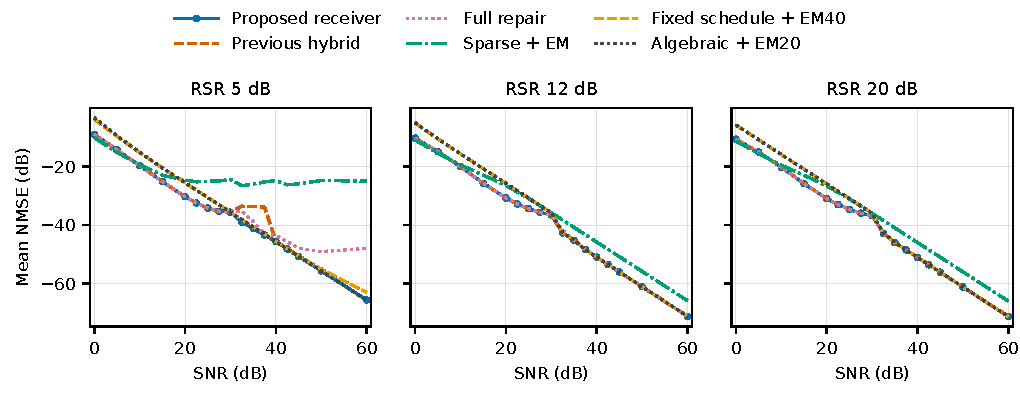
\includegraphics[width=\textwidth]{reliability_nmse.pdf}
\caption{Final channel-error comparison. Each point averages the three path-setting scores. Learned methods also average the scores from three training runs, not their channel estimates. All methods share observations. A fixed schedule and algebraic recovery both give strong high-SNR results.}
\label{fig:reliability-nmse}
\end{figure*}
\begin{figure*}[!t]
\centering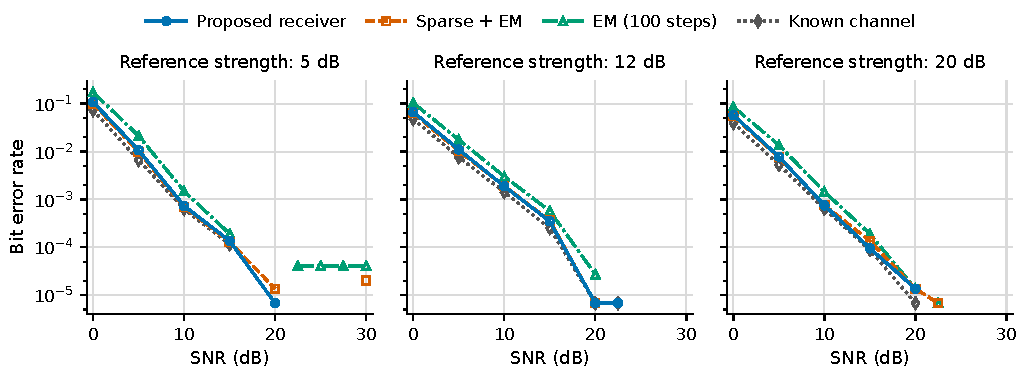
\includegraphics[width=\textwidth]{reliability_ber.pdf}
\caption{Bit error rate from 0 to 30~dB, averaged over the three path settings. All methods use the same data and detector. ``Known channel'' gives the detector the true channel. Points with no observed errors are omitted from the log scale, and lines break at those points. The supplement shows the full 0--60~dB range.}
\label{fig:reliability-ber}
\end{figure*}
Figure~\ref{fig:reliability-nmse} shows the full SNR range. Figure~\ref{fig:reliability-ber} focuses on the range where most bit errors occur. Zero observed errors cannot be drawn on a logarithmic axis and do not prove zero true BER. High-SNR results remain in Table~\ref{tab:reliability-regions} and the full-range supplementary plot.

\subsection{Where the Recovery Check Helps}
\begin{table*}[!t]
\centering
\caption{Results in three SNR ranges on the same final test data.}
\label{tab:reliability-regions}
\small
\setlength{\tabcolsep}{4pt}
\begin{tabular}{llrrrrr}
\toprule
Region & Metric & Proposed & \shortstack{Previous\\hybrid} & Full repair & Sparse/EM & Algebraic20 \\
\midrule
Ordinary (45) & dB & -20.242 & -20.242 & -20.242 & -18.964 & -15.470 \\
 & BER (\%) & 1.776440 & 1.776440 & 1.776440 & 1.662191 & 2.841254 \\
Weak target (24) & dB & -48.644 & -45.411 & -43.893 & -25.607 & -48.457 \\
 & BER (\%) & 0.000000 & 0.000000 & 0.000480 & 0.001441 & 0.000000 \\
High SNR (45) & dB & -56.744 & -56.512 & -54.638 & -44.052 & -56.754 \\
 & BER (\%) & 0.000000 & 0.000000 & 0.000196 & 0.000633 & 0.000000 \\
\bottomrule
\end{tabular}
\par\vspace{2pt}
\begin{minipage}{0.98\textwidth}\footnotesize Ordinary: SNR $\leq20$~dB, all references. Weak target: RSR 5~dB and SNR $>30$~dB. High SNR: SNR $\geq40$~dB, all references. These ranges overlap; their comparisons are descriptive. Zero BER means no observed bit errors, not proof of zero true error. The first three methods give exactly the same estimates in the ordinary range.\end{minipage}
\end{table*}

The recovery check targets reference 5~dB and SNR above 30~dB: 24 settings. Here the mean NMSE is $-48.644$~dB. The gain is 3.232~dB over the previous hybrid, with descriptive interval $[2.249,3.966]$~dB, and 4.750~dB over the full repair, with interval $[1.836,5.326]$~dB. The check triggers on about 26.7--27.0\% of target cases across training runs. Every triggered alternative is accepted in this test, and none has an invalid design.

Fifteen of the 153 setting means improve over the previous hybrid; the rest are equal. No setting mean is worse, though individual channel errors can be worse. All outputs at SNR at most 20~dB, and all cases outside the new check, remain exactly unchanged. Both methods have zero observed bit errors in the target range. The large channel-error gain therefore gives no measured BER gain there.

The proposed receiver is worse than the full repair in 32 setting means. Eight pointwise intervals exclude zero; these are descriptive comparisons, not simultaneous findings across all settings. The largest loss is 0.701~dB at two paths, reference 20~dB and SNR 32.5~dB, outside the new check. At strong references and SNR at least 40~dB, mean NMSE is $-58.555$~dB versus $-58.558$~dB for the full repair. We retain these losses rather than retune on the final test.

Algebraic-plus-EM20 is close to the proposed receiver in the target range ($-48.457$~dB) and is the fastest full pipeline in the table. Across the full grid, however, its BER is 0.835676\%. This supports combining the methods while showing that learning is not needed for accurate high-SNR recovery. Sparse/EM's BER advantage is concentrated in ordinary-SNR operation, which the new check preserves rather than improves.

\subsection{Runtime and Remaining Limits}
The proposed receiver passes both required p90 checks in both timing runs. Full-grid times are 4.282 and 7.254~ms; target-range times are 4.162 and 7.031~ms. The table reports the slower run. The second run is also slower for the baselines. The full repair passes in the first but fails in the second, at 14.690~ms overall and 14.858~ms in the target range.

The proposed receiver's maximum times are 5.225 and 22.276~ms. One of 1,377 calls in the second run exceeds 10.74~ms, even though its recovery check does not trigger. The measurements do not identify the cause. Passing the p90 target is therefore different from meeting a deadline on every call.

Earlier tests found that strong learned filtering can cause bias when noise is very small, and that wrong noise or reference-phase inputs can increase error. The final receiver has not been validated under these errors. Correct reference phase, correct variance, Gaussian fitting pilots and the stated linear-array model remain assumptions. Tests on atomic hardware, other user counts, other array shapes and coded communication links remain future work.
